\section{The canonical DR-plan}
\label{sec:DRP}

\subsection{Theory}

% In the problem of the optimal DR-Plan there is generally not a unique plan.
% % Indeed, we will prove a union of $N$ well-constrained subgraphs will result in $N$ unique plans, but that at the $N^{\text{th}}$ level of the tree it will always be the same. Therefore, all choices of decomposition are in some sense equivalent. The theorem we seek to prove is thus:
% However, we will show that regardless of which children are chosen for the plan, so long as they satisfy the definition of an optimal DR-plan, the recombination will require solving of the same systems. Being the smallest such structure that offers this, the definition of an optimal DR-plan could be considered the canonical DR-plan.
% % To assist in showing this, we prove this core theorem throughout this section:

% In this section, we discuss 2D bar-joint graphs. All vertex weights are $2$, all edge weights are $1$, and constant $k= -{{3}\choose{2}}=-3$. Trivial graphs are a single vertex and empty set. Furthermore, 2D well-constrained graphs must be connected.
% % The greatest density of a 2D well-constrained graph is $-2$ (the vertex). The other disconnected part of the graph would need to have a density of $-1$, which is over-constrained and not possible in a well-constrained graph (because there is no trivial graph with that density).

In the problem of the optimal DR-Plan there is generally not a unique plan. Furthermore, there is no obvious way to find the optimal plan. In this section we present a particular way to construct a plan that guarantees optimality. We call this the \dfn{canonical} plan.

\begin{definition}
    The \dfn{canonical DR-plan} is a DR-plan that satisfies the following two properties:
    \begin{enumerate}
        \item Children are isostatic vertex-maximal subgraphs of the parent.
        \item All of the isostatic vertex-maximal subgraphs are children if any two of them intersect trivially, otherwise exactly two are children.
    \end{enumerate}
\end{definition}


The importance of this formulation is stated succinctly in the following theorem.

\begin{theorem}\label{theorem:canonical_is_optimal}
    A canonical DR-plan is an optimal DR-plan.
\end{theorem}

The proof of this theorem is a direct result of this more general theorem.

\begin{theorem}\label{theorem:main}
Given an isostatic 2D bar-joint graph $G$ and $\comdrp{G}$, for all nodes $C$ with children $C_1,\ldots,C_N$ keep children according to the following rules.
\begin{enumerate}
    \item If $C_i \cap C_j$ is trivial then keep all $C_1,\ldots,C_N$ as children.
    \item If $C_i \cap C_j$ is isostatic then select any two out of $C_1,\ldots,C_N$ as children.
\end{enumerate}
This covers all cases and the resulting plan is an optimal DR-plan.
\end{theorem}

\begin{remark}
    \todo{Someone} \uncited discuss cluster minimality as a desirable property for children in a DR-plan. The canonical DR-plan in this paper intrinsically satisfies this property. If the children were not cluster minimal, then the union of children that form a larger cluster is itself isostatic and the original children were not vertex-maximal.
\end{remark}

This theorem (proven in the Appendix) relies on the following crucial observations and lemmas.

\begin{observation}\label{lemma:union_intersection}
If $F_i$ and $F_j$ are well-constrained subgraphs of the same well-constrained graph $F$, then it must be that: (1) $F_i\cup F_j$ is not trivial; (2) $F_i\cup F_j$ is under-constrained if and only if $F_i\cap F_j$ is trivial; (3) $F_i\cup F_j$ is well-constrained if and only if $F_i\cap F_j$ is well-constrained; and (4) $F_i\cap F_j$ is not under-constrained.
\end{observation}

\begin{lemma}\label{lemma:wc_intersection_is_C}
$C_i\cup C_j$ is well-constrained if and only if $C_i\cup C_j = C$.
\end{lemma}

\begin{lemma}\label{lemma:wc_intersection_makes_all_wc}
If $C_i\cup C_j$ is well-constrained, then $\forall k: C_i\cup C_k$ is well-constrained.
Alternatively, if $C_i\cup C_j=C$, then $\forall k: C_i\cup C_k=C$.
\end{lemma}

\begin{lemma}\label{lemma:uc_intersection_makes_all_uc}
If $C_i\cap C_j$ is trivial, then $\forall k: C_i\cap C_k$ is trivial.
\end{lemma}







\begin{figure*}\centering
\begin{subfigure}{.3\linewidth}\centering
    % \newcommand{\tedge}[5]{\draw[#3] (#1)-- node[e, #5] (e#4) {#4} (#2)}

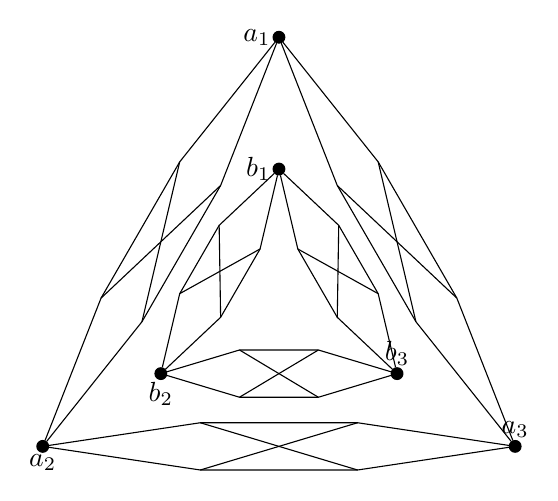
\begin{tikzpicture}[scale=3]
    \tikzstyle{v}=[draw, circle, minimum size=0.75cm]
    \tikzstyle{c}=[draw, circle, inner sep=1.5, fill=black]
    \tikzstyle{e}=[]

    \node[circle,fill=white,inner sep=7] (center) at (0,0-.125-.1) {};

    \node[c] (v1) at (0,0.866) [label={left,inner sep=.555}:$a_1$]{};
    \node[c] (v2) at (-1,-0.866) [label={below,inner sep=.555}:$a_2$]{};
    \node[c] (v3) at (1,-0.866) [label={above,inner sep=.555}:$a_3$]{};

    \node[c] (v4) at (0,0.433-.125) [label={left,inner sep=.555}:$b_1$]{};
    \node[c] (v5) at (-0.5,-0.433-.125) [label={below,inner sep=.555}:$b_2$]{};
    \node[c] (v6) at (0.5,-0.433-.125) [label={above,inner sep=.555}:$b_3$]{};

    \tedge{v1}{v2}{solid}{}{};
    \tedge{v1}{v3}{solid}{}{};
    \tedge{v2}{v3}{solid}{}{};

    \tedge{v4}{v5}{solid}{}{};
    \tedge{v4}{v6}{solid}{}{};
    \tedge{v5}{v6}{solid}{}{};


    \tedge{v1}{v4}{solid}{}{};
    \tedge{v2}{v5}{solid}{}{};
    \tedge{v3}{v6}{solid}{}{};


    \tedge{v4}{center}{dashed}{}{};
    \tedge{v5}{center}{dashed}{}{};
    \tedge{v6}{center}{dashed}{}{};


    % sin(30deg) = 0.5
    % cos(30deg) = 0.866

    % o/i -> outside/inside triangle
    % b/l/r -> bottom/left/right edge of triangle

    \coordinate (ob0) at (-0.333,-0.866-0.1);
    \coordinate (ob1) at (0.333,-0.866-0.1);
    \coordinate (ob2) at (-0.333,-0.866+0.1);
    \coordinate (ob3) at (0.333,-0.866+0.1);
    \draw (v2) -- (ob0) -- (ob1) -- (v3);
    \draw (v2) -- (ob2) -- (ob3) -- (v3);
    \draw (ob0) -- (ob3);
    \draw (ob2) -- (ob1);

    \draw[rotate around={60:(-1,-0.866)}] (v2) -- (-0.333,-0.766) -- (0.333,-0.766) -- (v1);
    \draw[rotate around={60:(-1,-0.866)}]  (v2) -- (-0.333,-0.966) -- (0.333,-0.966) -- (v1);
    \draw[rotate around={60:(-1,-0.866)}]  (-0.333,-0.766) -- (0.333,-0.966);
    \draw[rotate around={60:(-1,-0.866)}]  (-0.333,-0.966) -- (0.333,-0.766);

    \draw[rotate around={-60:(1,-0.866)}] (v3) -- (0.333,-0.766) -- (-0.333,-0.766) -- (v1);
    \draw[rotate around={-60:(1,-0.866)}]  (v3) -- (0.333,-0.966) -- (-0.333,-0.966) -- (v1);
    \draw[rotate around={-60:(1,-0.866)}]  (-0.333,-0.766) -- (0.333,-0.966);
    \draw[rotate around={-60:(1,-0.866)}]  (-0.333,-0.966) -- (0.333,-0.766);




    \coordinate (ib0) at (-0.167,-0.433-.125-0.1); %(-.167,-.658)
    \coordinate (ib1) at (0.167,-0.433-.125-0.1); %(.167,-.658)
    \coordinate (ib2) at (-0.167,-0.433-.125+0.1);%(-.167,-.458)
    \coordinate (ib3) at (0.167,-0.433-.125+0.1);%(.167,-.458)
    \draw (v5) -- (ib0) -- (ib1) -- (v6);
    \draw (v5) -- (ib2) -- (ib3) -- (v6);
    \draw (ib0) -- (ib3);
    \draw (ib2) -- (ib1);

    \draw[rotate around={60:(-0.5,-0.558)}] (v5) -- (-.167,-.658) -- (.167,-.658) -- (v4);
    \draw[rotate around={60:(-0.5,-0.558)}]  (v5) -- (-.167,-.458) -- (.167,-.458) -- (v4);
    \draw[rotate around={60:(-0.5,-0.558)}]  (-.167,-.658) -- (.167,-.458);
    \draw[rotate around={60:(-0.5,-0.558)}]  (-.167,-.458) -- (.167,-.658);

    \draw[rotate around={-60:(0.5,-0.558)}] (v6) -- (.167,-.658) -- (-.167,-.658) -- (v4);
    \draw[rotate around={-60:(0.5,-0.558)}]  (v6) -- (.167,-.458) -- (-.167,-.458) -- (v4);
    \draw[rotate around={-60:(0.5,-0.558)}]  (-.167,-.658) -- (.167,-.458);
    \draw[rotate around={-60:(0.5,-0.558)}]  (-.167,-.458) -- (.167,-.658);
% \newcommand{\tedge}[5]{\draw[#3] (#1)-- node[e, #5] (e#4) {#4} (#2)}

    % \draw (-1,-0.866) -- (-0.333,-0.966);

\end{tikzpicture}

    \caption{}\label{fig:c2c3ofk33s:a}
\end{subfigure}%
\begin{subfigure}{.7\linewidth}\centering
    % \newcommand{\tedge}[5]{\draw[#3] (#1)-- node[e, #5] (e#4) {#4} (#2)}

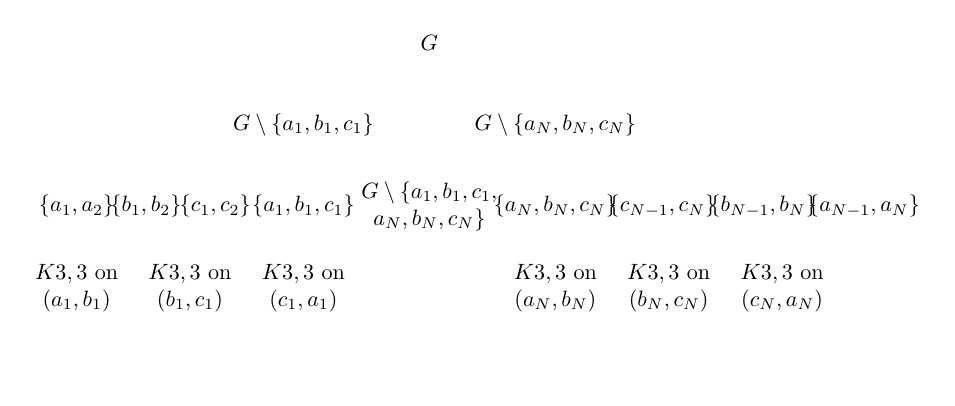
\begin{tikzpicture}[scale=.8, transform shape]
    \tikzstyle{v}=[draw, circle, minimum size=0.75cm, font=\footnotesize]
    % \tikzstyle{b}=[draw, font=\footnotesize]
    \tikzstyle{b}=[align=center]
    \tikzstyle{e}=[]

    \node[b] (c0) at (0,0*1.3) {$G$};
    \node[b] (c1a) at (-2,-1*1.3) {$G\setminus\{a_1,b_1,c_1\}$};
    \node[b] (c1b) at (2,-1*1.3) {$G\setminus\{a_N,b_N,c_N\}$};
    \node[b] (c2b) at (0,-2*1.3) {$G\setminus\{a_1,b_1,c_1,$ \\ $a_N,b_N,c_N\}$};
    \node[b] (c2a) at (-2,-2*1.3) {$\{a_1,b_1,c_1\}$};
    \node[b] (c2c) at (2,-2*1.3) {$\{a_N,b_N,c_N\}$};
    \node[b] (c2ab1) at (-5.6,-2*1.3) {$\{a_1,a_2\}$};
    \node[b] (c2ab2) at (-4.5,-2*1.3) {$\{b_1,b_2\}$};
    \node[b] (c2ab3) at (-3.4,-2*1.3) {$\{c_1,c_2\}$};
    \node[b] (c2bc1) at (6.9,-2*1.3) {$\{a_{N-1},a_N\}$};
    \node[b] (c2bc2) at (5.3,-2*1.3) {$\{b_{N-1},b_N\}$};
    \node[b] (c2bc3) at (3.7,-2*1.3) {$\{c_{N-1},c_N\}$};

    \node[b] (ab1k33) at (-5.6,-3*1.3) {$K3,3$ on \\ $(a_1,b_1)$};
    \node[b] (bc1k33) at (-7.6/2,-3*1.3) {$K3,3$ on \\ $(b_1,c_1)$};
    \node[b] (ca1k33) at (-2,-3*1.3) {$K3,3$ on \\ $(c_1,a_1)$};

    \node[b] (abNk33) at (2,-3*1.3) {$K3,3$ on \\ $(a_N,b_N)$};
    \node[b] (bcNk33) at (7.6/2,-3*1.3) {$K3,3$ on \\ $(b_N,c_N)$};
    \node[b] (caNk33) at (5.6,-3*1.3) {$K3,3$ on \\ $(c_N,a_N)$};


    \node[b] (c3a) at (-2,-4*1.3) {};
    \node[b] (c3b) at (2,-4*1.3) {};


    \tedge{c0}{c1a}{solid}{}{};
    \tedge{c0}{c1b}{solid}{}{};

    \tedge{c1a}{c2ab1}{solid}{}{};
    \tedge{c1a}{c2ab2}{solid}{}{};
    \tedge{c1a}{c2ab3}{solid}{}{};
    \tedge{c1a}{c2a}{solid}{}{};
    \tedge{c1a}{c2b}{solid}{}{};

    \tedge{c1b}{c2bc1}{solid}{}{};
    \tedge{c1b}{c2bc2}{solid}{}{};
    \tedge{c1b}{c2bc3}{solid}{}{};
    \tedge{c1b}{c2b}{solid}{}{};
    \tedge{c1b}{c2c}{solid}{}{};

    \tedge{c2a}{ab1k33}{solid}{}{};
    \tedge{c2a}{bc1k33}{solid}{}{};
    \tedge{c2a}{ca1k33}{solid}{}{};
    \tedge{c2c}{abNk33}{solid}{}{};
    \tedge{c2c}{bcNk33}{solid}{}{};
    \tedge{c2c}{caNk33}{solid}{}{};

    \tedge{c2b}{c3a}{dashed}{}{};
    \tedge{c2b}{c3b}{dashed}{}{};
\end{tikzpicture}

    \caption{}\label{fig:c2c3ofk33s:b}
\end{subfigure}

\caption{(\ref{fig:c2c3ofk33s:a}) A doublet ($C_2 \times C_3$) with each edge of the triangles replaced by a $K_{3,3}$. This pattern continues inwards for a total of $N$ triangles, indicated by the dashed lines. (\ref{fig:c2c3ofk33s:b}) Most of the DR-plan of this graph, omitting further decomposition of $K_{3,3}$ subgraphs into the separate 9 edges and of edges into the component nodes. $G\setminus\{a_i,b_i,c_i\}$ is shorthand for $G$ difference those nodes and all of the nodes in the corresponding $K_{3,3}$ subgraphs. The dashed lines indicated that this exact structure is repeated.}
\label{fig:c2c3ofk33s}
\end{figure*}

\myexample
\textsl{[DR-Plan for self-similar structure]}
This section details the canonical decomposition of the graph in Figure \ref{fig:c2c3ofk33s}. The graph $G$ has only two isostatic vertex-maximal subgraphs, $G$ without the outermost triangle composed of $K_{3,3}$ graphs (triangle $1$) and $G$ without the inner triangle $N$. These intersect on $G$ without triangle $1$ and $N$ which is clearly well-constrained. As explained in the proof of Theorem \ref{theorem:main}, part 2, since there are only 2 possible children, their intersection must be a node 2 levels below the parent. Just as expected, it is on the third level, as it is a child of both of $G$'s children. Furthermore, it intersects trivially with the edges that connect triangle $1$ and $N$ to $2$ and $N-1$, respectively; these necessarily intersect with triangle $1$ and $N$ themselves trivially (by Theorem \ref{theorem:main}, part 1) making all of these children. The triangles then decompose into their constituent $K_{3,3}$ graphs, which then decompose into 9 edges.

Now, the self-similar nature of the graph is clear; $G$ without triangle $1$ and $N$ has the same structure, and thus the same pattern is repeated until only triangle $(N+1)/2$ remains in the case that $N$ is odd, or until only triangles $N/2$ and $N/2+1$ remain if $N$ is even.


% \begin{example}
%     In
% \end{example}




% \subsection{Extensions}
% This framework immediately pushes through for body-pin systems via a simple reduction. If there are $N$ pins on a body, it can be represented as a 2-tree with $N$ vertices, each corresponding to a pin, making sure to select edge distances such that the distance between pins is preserved. E.g.\ a body with two pins is an edge, three pins is a triangle, etc. Any bodies that share a pin now intersect on their vertex that corresponds to that pin. Now we have a bar-joint representation of the body-pin system in 2D and all proofs follow.

% With more effort, it can be shown that pinned line-incidence systems can also use this framework. This is done in section \ref{XXX}.


\subsection{Algorithm}

The first step of the algorithm to find an optimal DR-plan is the most difficult --- to find the well-constrained vertex-maximal proper subgraphs of the input well-constrained graph. There are two approaches: (1) the bottom-up approach, using the Frontier algorithm \cite{Oung:2001:FFE:376957.376995} to grow these components from single vertices; and (2) the top-down approach, using the pebble game algorithm \cite{Jacobs:1997:PG} on each node and taking the largest components that are not subgraphs of any larger ones. After the subgraphs have been found, it is a straightforward application of the theory. If the intersection of any two of the subgraphs is well-constrained, then take those two to be children of the graph. Otherwise, all the subgraphs are the children. Apply recursively to the children. This naturally terminates when you reach trivial subgraphs. The complexity of this depends on the algorithm for finding children (both are polynomial) and the depth of the plan (the deeper the plan, i.e.\ the smaller the max fan-in, the longer the running time). \todo{Think more about complexity.}
